 
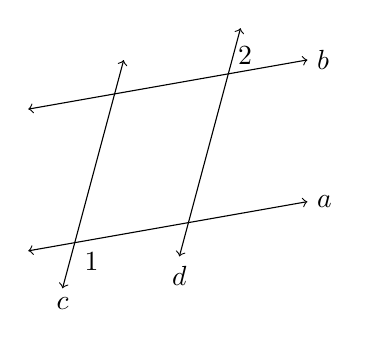
\begin{tikzpicture}[scale=0.6]
\draw[<->](0,0)--++(10:6)node[anchor=west]{$a$}; 
\draw[<->](0,3)--++(10:6)node[anchor=west]{$b$};
\draw[<->](0,0)++(10:1)node[anchor=north west]{$1$}++(75:-1)node[anchor=north]{$c$}--++(75:5);
\draw[<->](0,3)++(10:4.3)node[anchor=south west]{$2$}++(75:-4)node[anchor=north]{$d$}--++(75:5);
\end{tikzpicture}\\
In the figure above, lines $a$ and $b$ are parallel to each other, as are lines $c$ and $d$.  If $m\angle 2=65\degree$, what is the measure of $\angle 1$?


\ifsat
	\begin{enumerate}[label=\Alph*)]
		\item $ 25\degree$ 
		\item $ 50\degree$ 
		\item $ 65\degree$ 
		\item $ 115\degree$ % 
	\end{enumerate}
\else
\fi

\ifacteven
	\begin{enumerate}[label=\textbf{\Alph*.},itemsep=\fill,align=left]
		\setcounter{enumii}{5}
		\item $ 25\degree$ 
		\item $ 50\degree$ 
		\item $ 65\degree$ 
		\addtocounter{enumii}{1}
		\item $ 115\degree$ % 
		\item None of these. 
	\end{enumerate}
\else
\fi

\ifactodd
	\begin{enumerate}[label=\textbf{\Alph*.},itemsep=\fill,align=left]
		\item $ 25\degree$ 
		\item $ 50\degree$ 
		\item $ 65\degree$ 
		\item $ 115\degree$ % 
		\item None of these. 
	\end{enumerate}
\else
\fi

\ifgridin
 $ 115\degree$ % 

\else
\fi

